\documentclass{article}
\usepackage[normalem]{ulem}
\usepackage[utf8]{inputenc}
\usepackage{graphicx}
\usepackage{mathtools}
\usepackage{amssymb}
\usepackage{amsmath}
\usepackage{macros}
\usepackage{color}

\begin{document}
\section{Pappos-guldins regel för rotationsvolymer}
% img 1
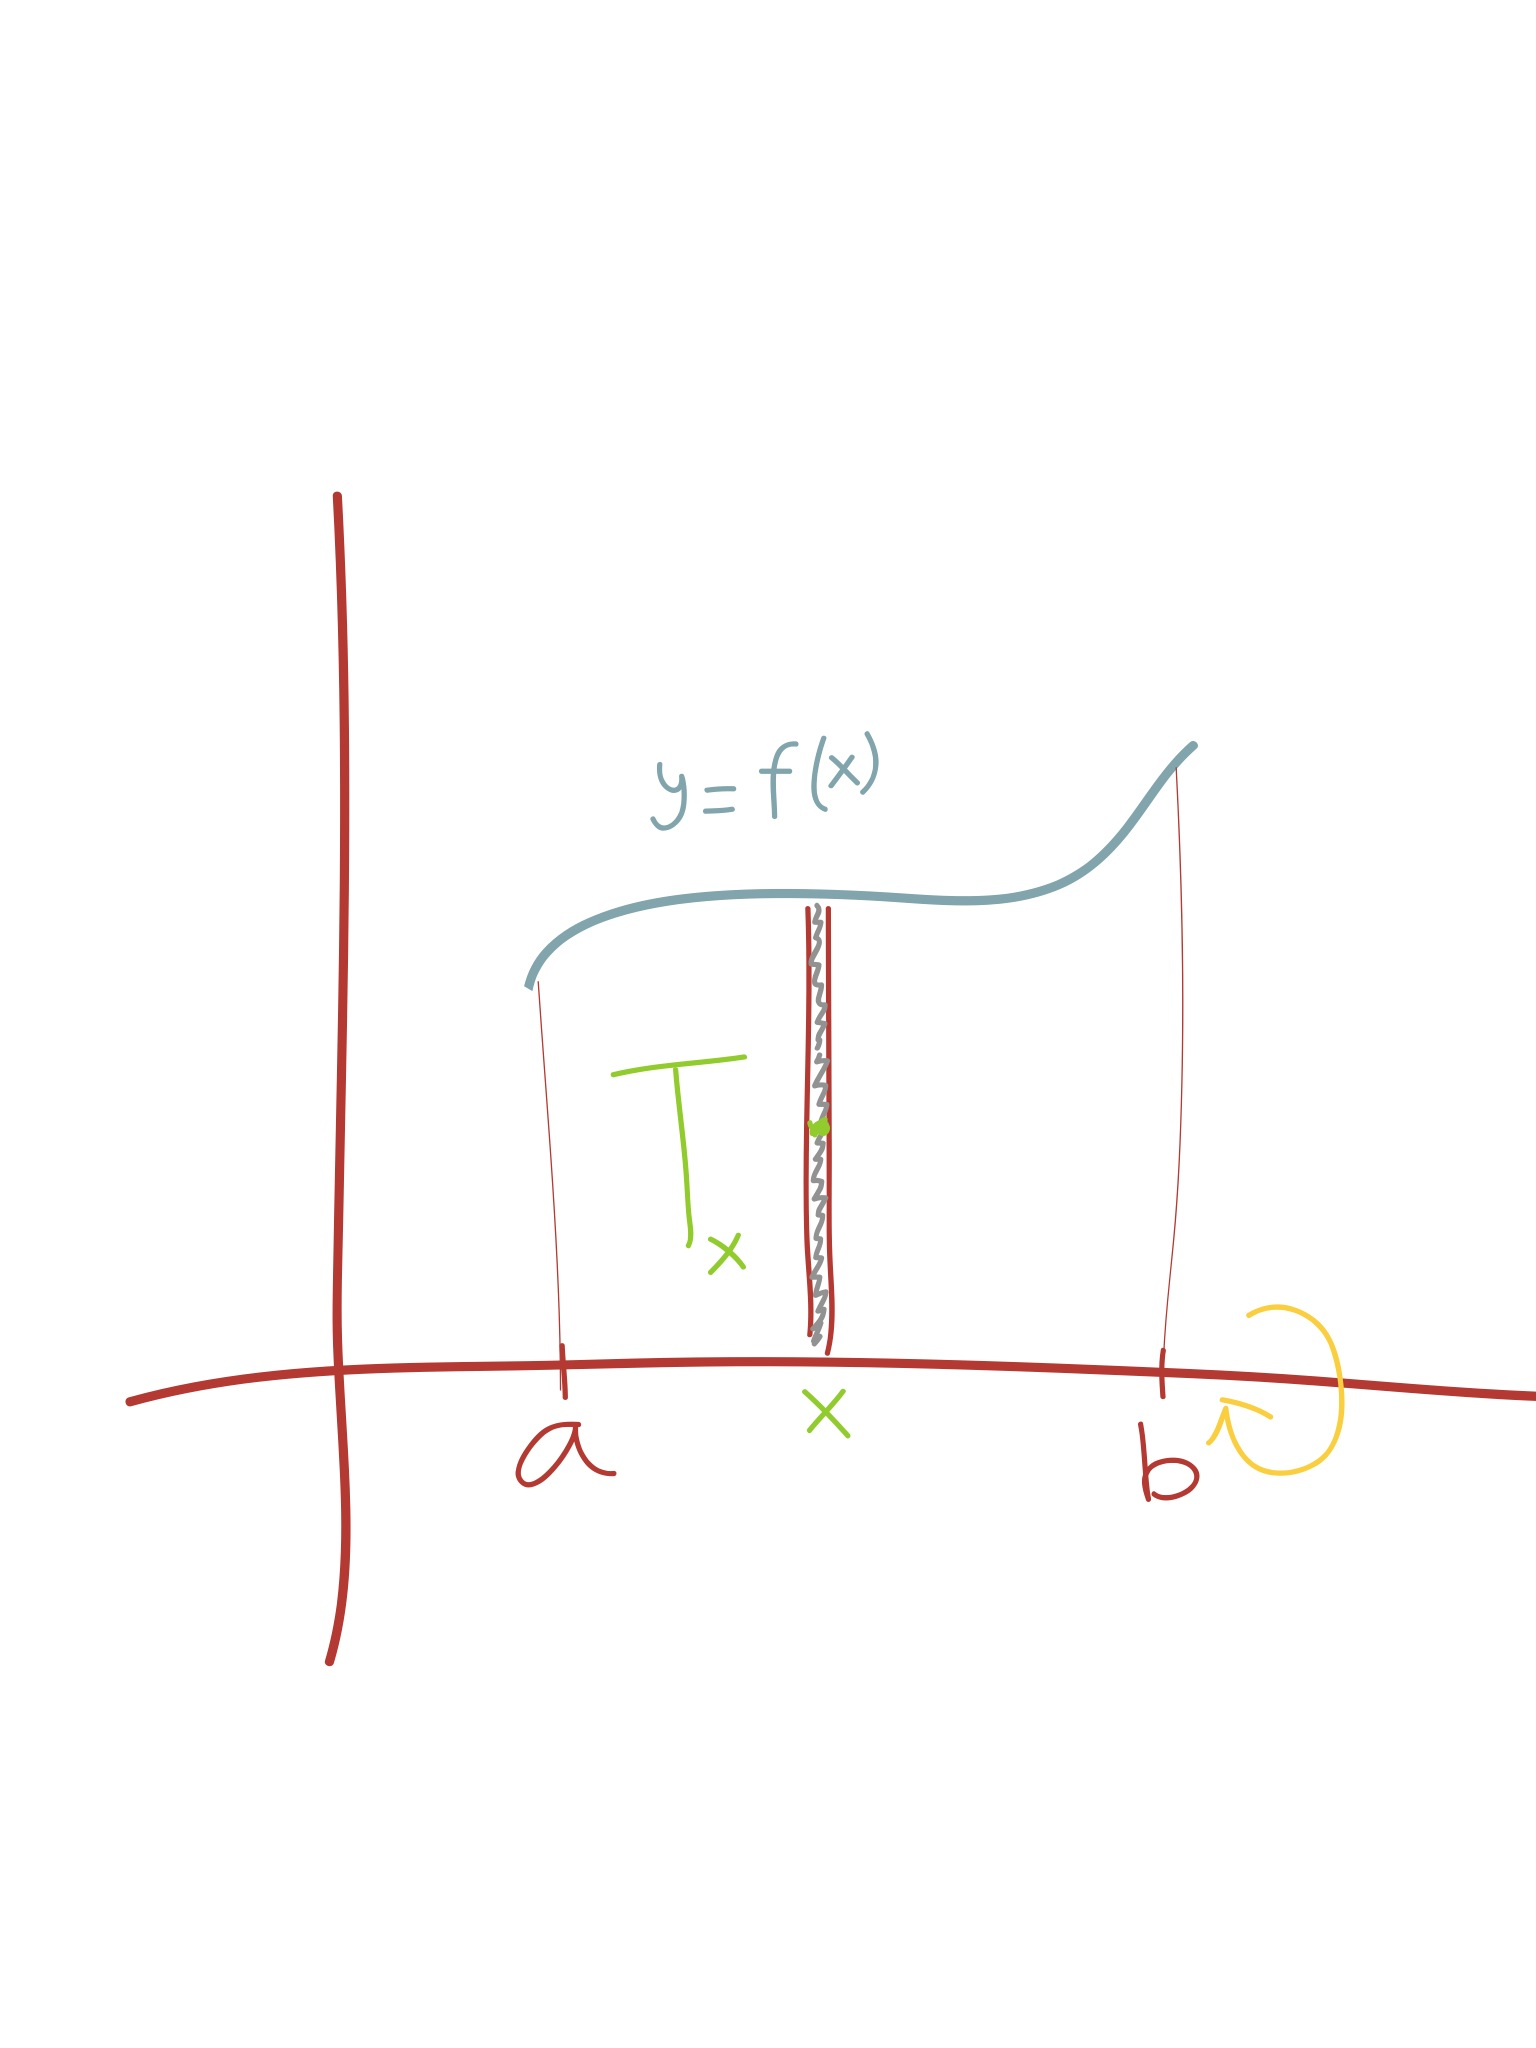
\includegraphics[scale=0.10]{img/img1.jpg}
% img 2?
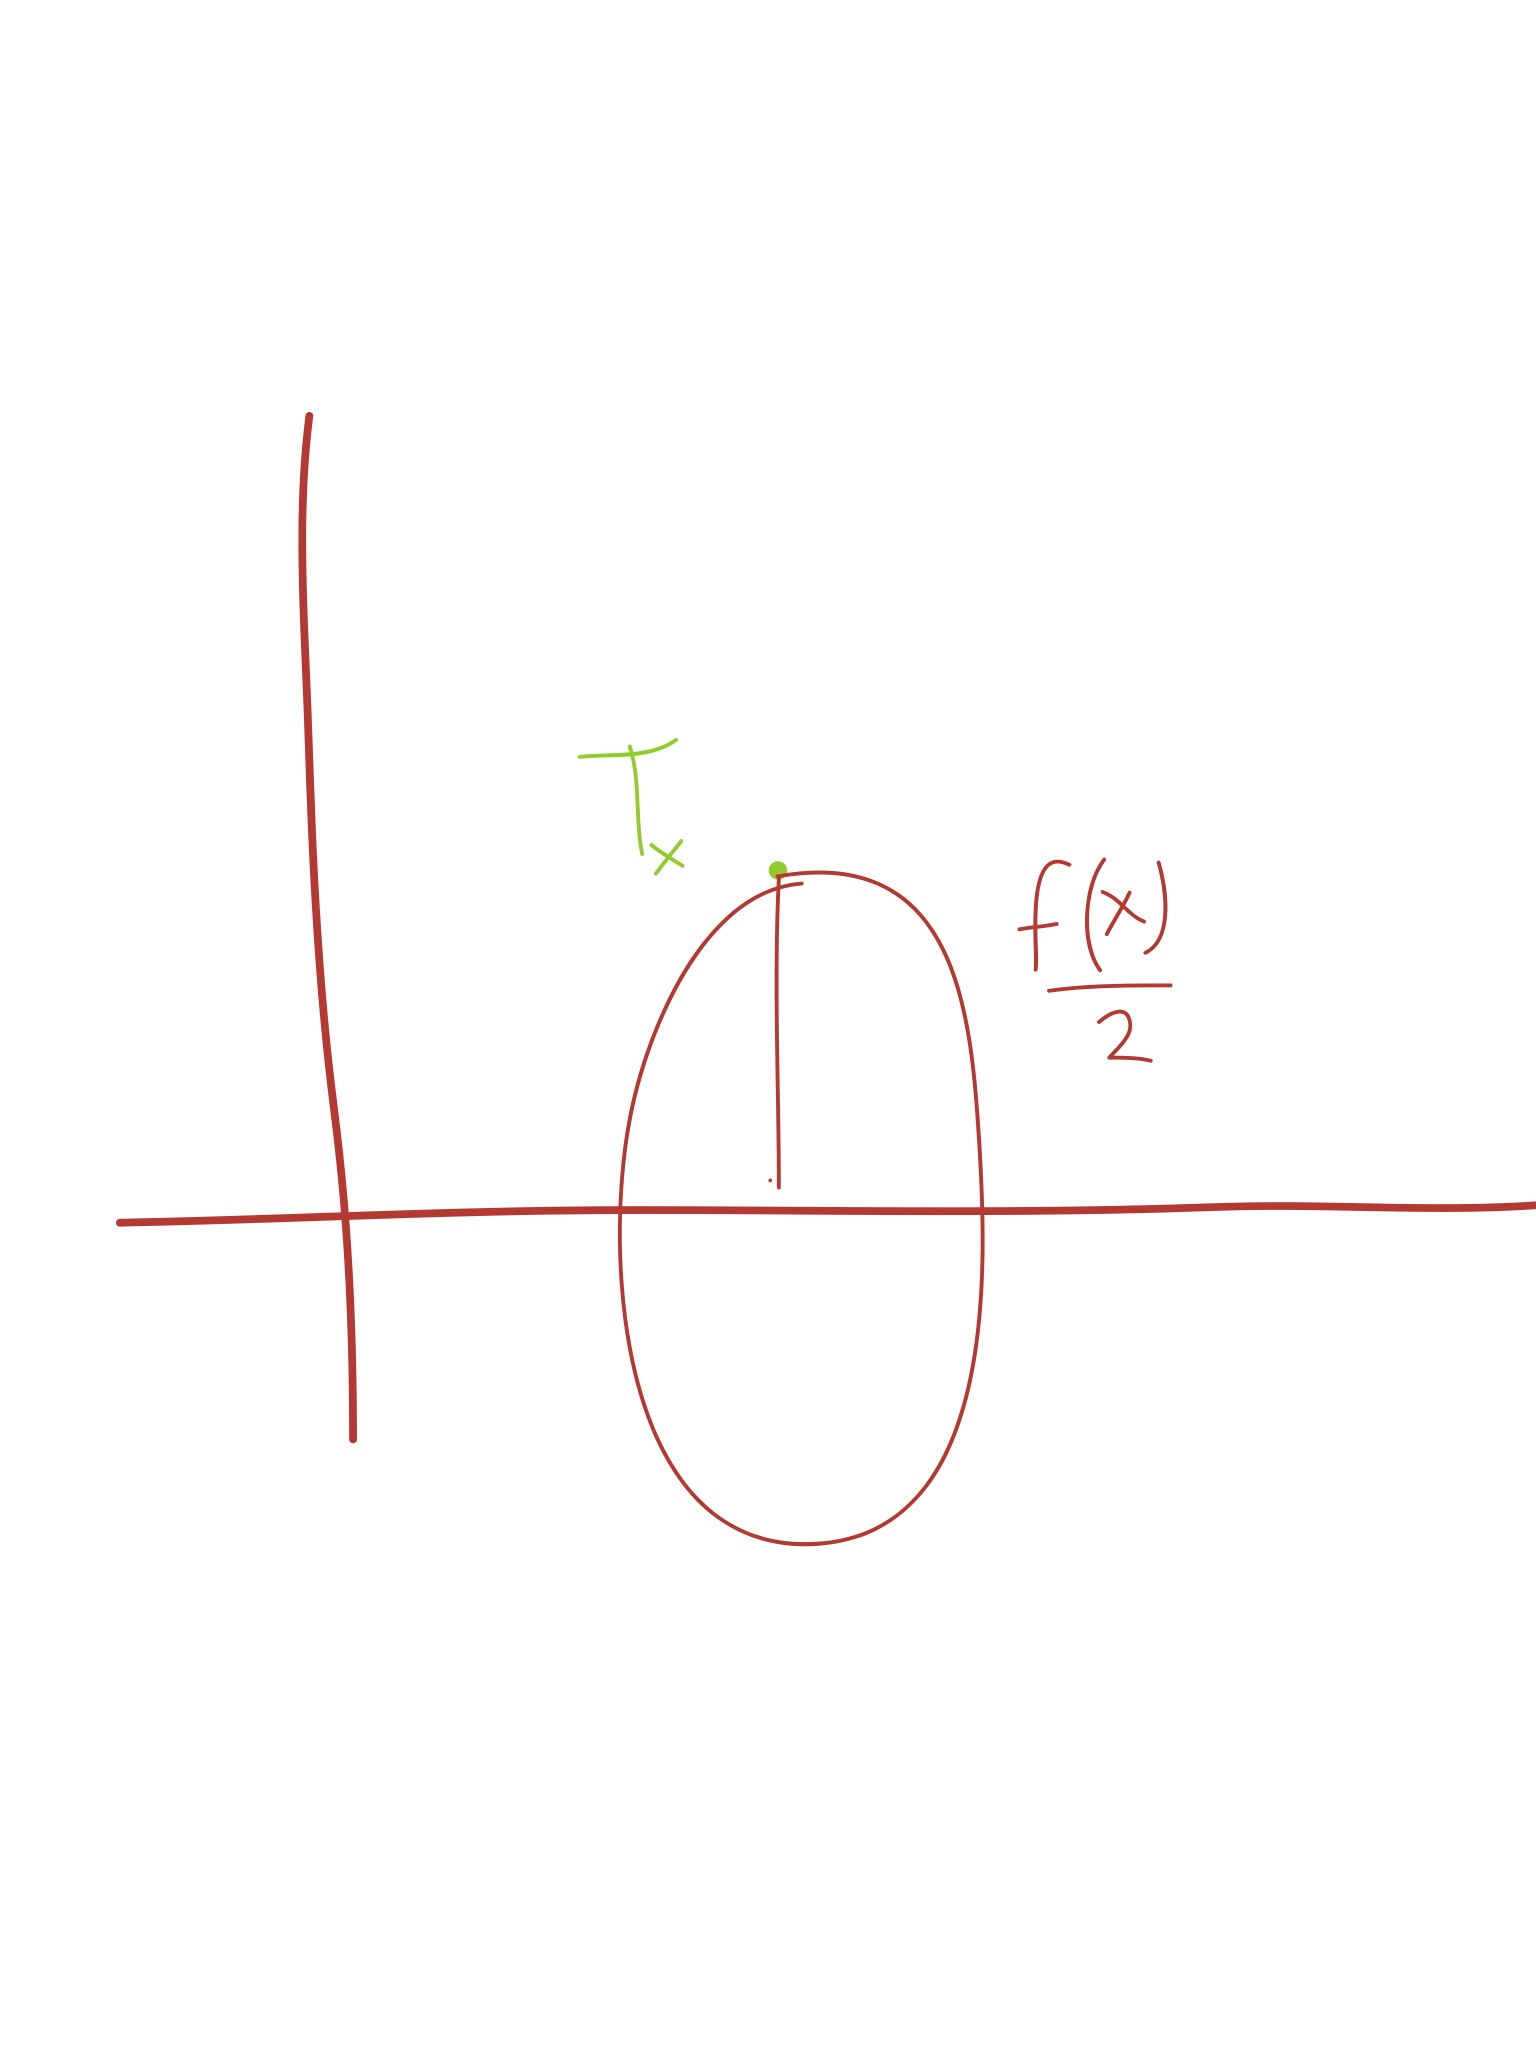
\includegraphics[scale=0.10]{img/img2.jpg}
$$ D=\{ (x,y) : a\le x\le b, 0\le y\le f(x) \} $$
$$ A(x) = \pi f^2(x) $$
$$ dV = \pi f^2(x)\ dx; T_x=(x, \f{f(x)}2) $$
$$ dV = 2\pi \f{f(x)}2 f(x)\ dx $$

% img 3
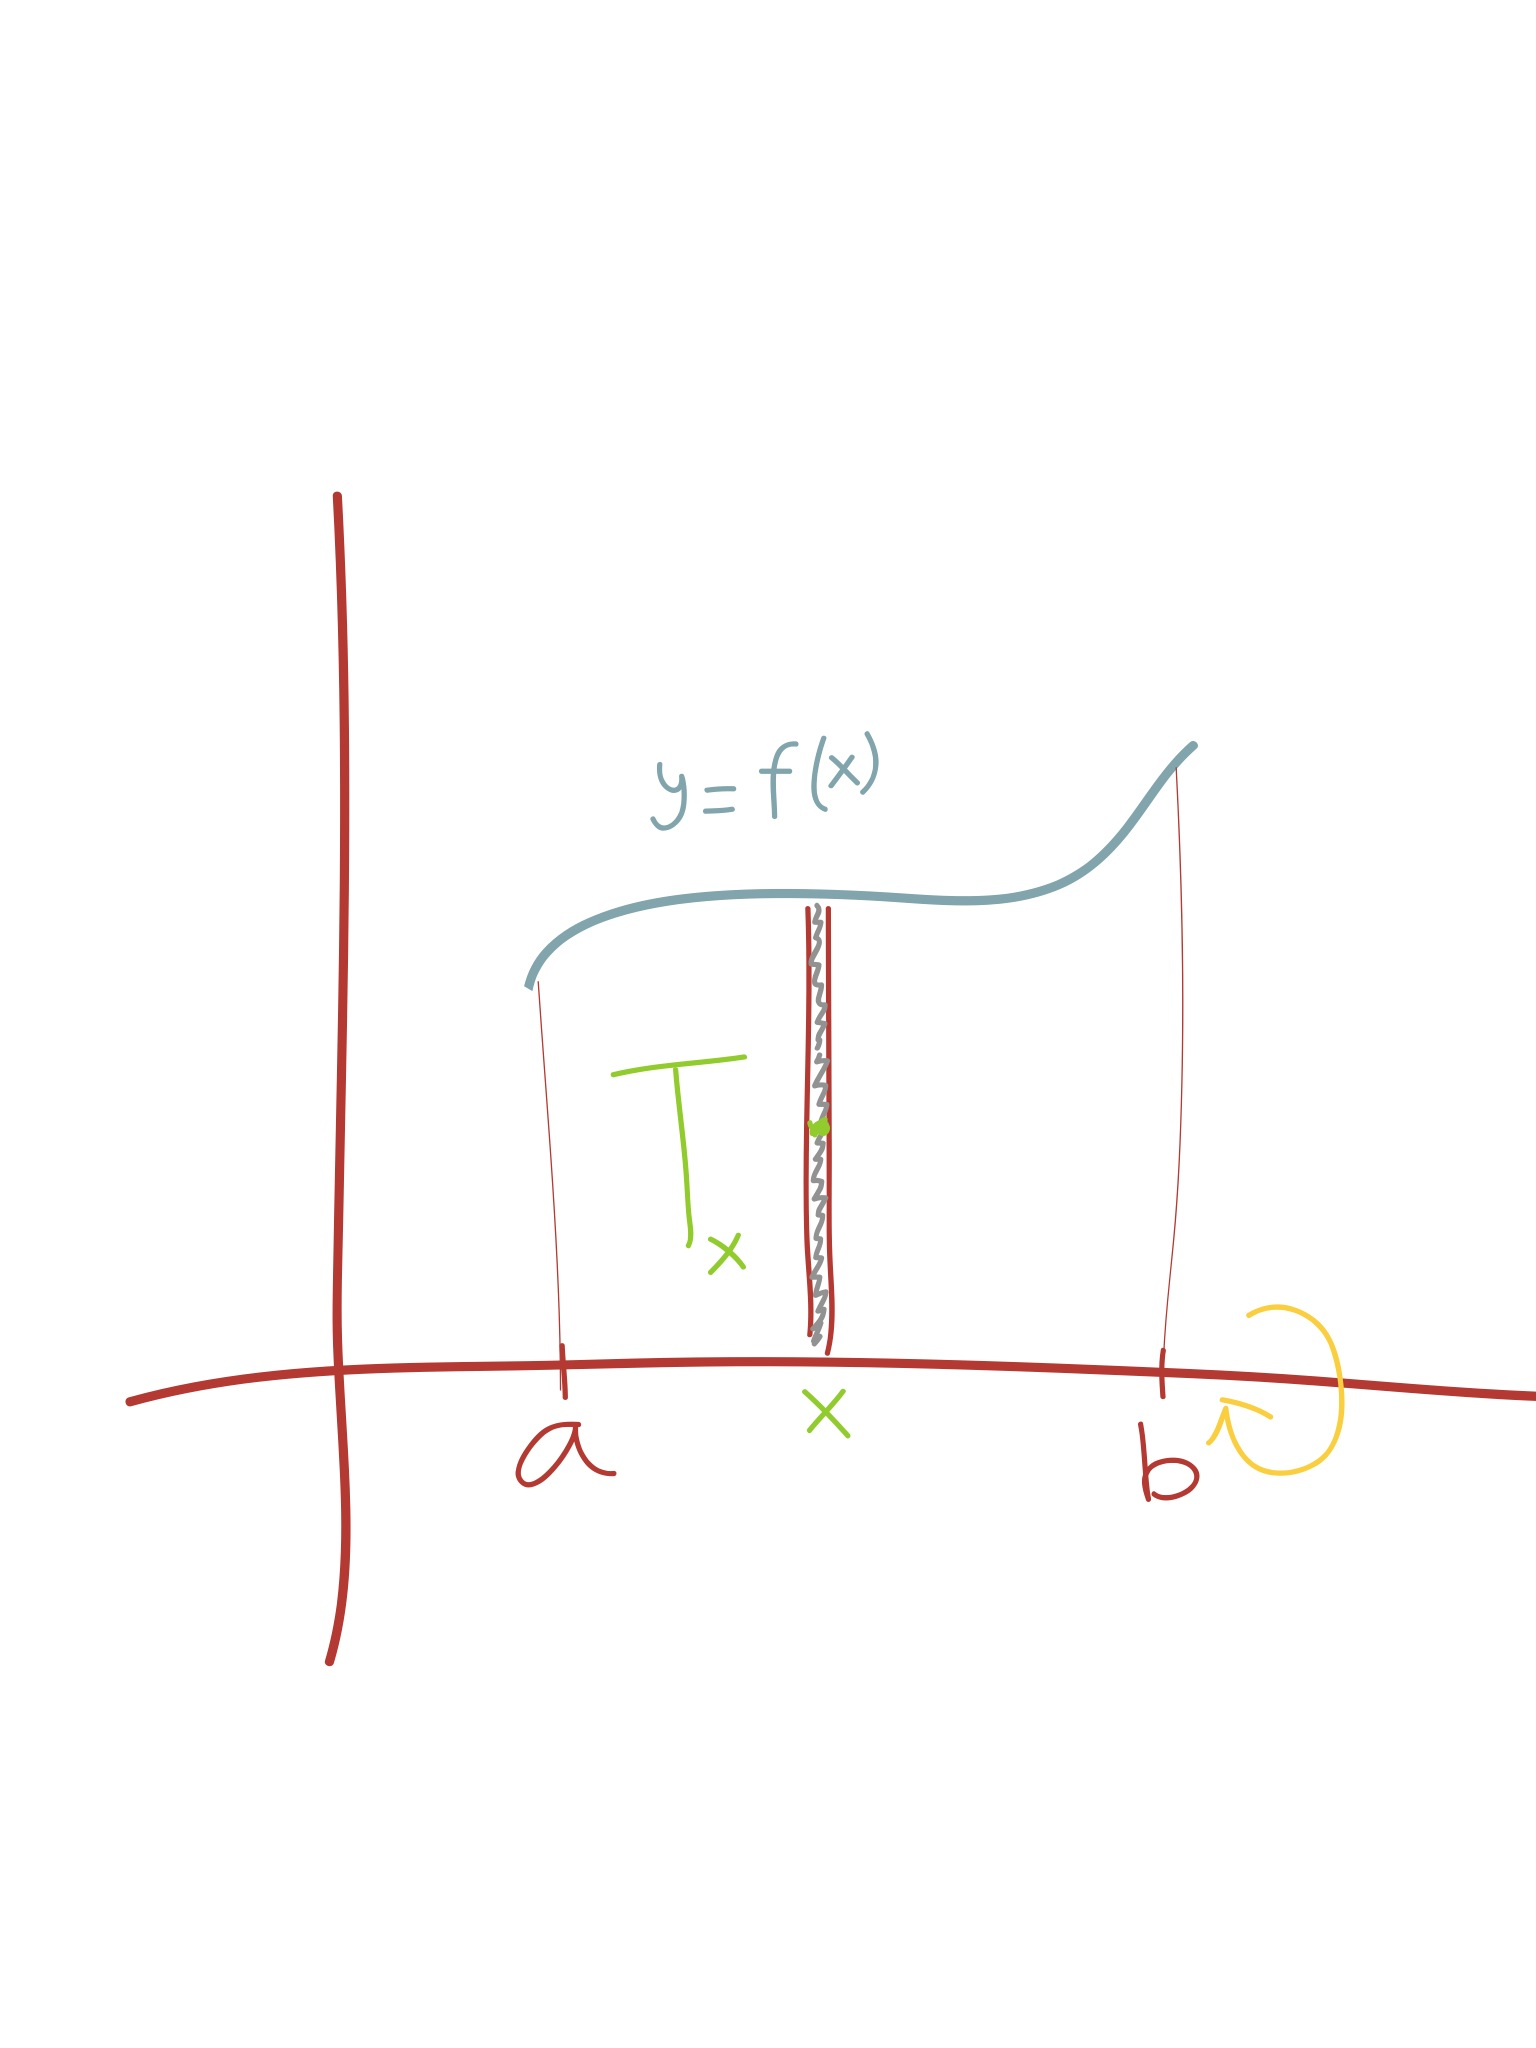
\includegraphics[scale=0.10]{img/img1.jpg}
% img 4?
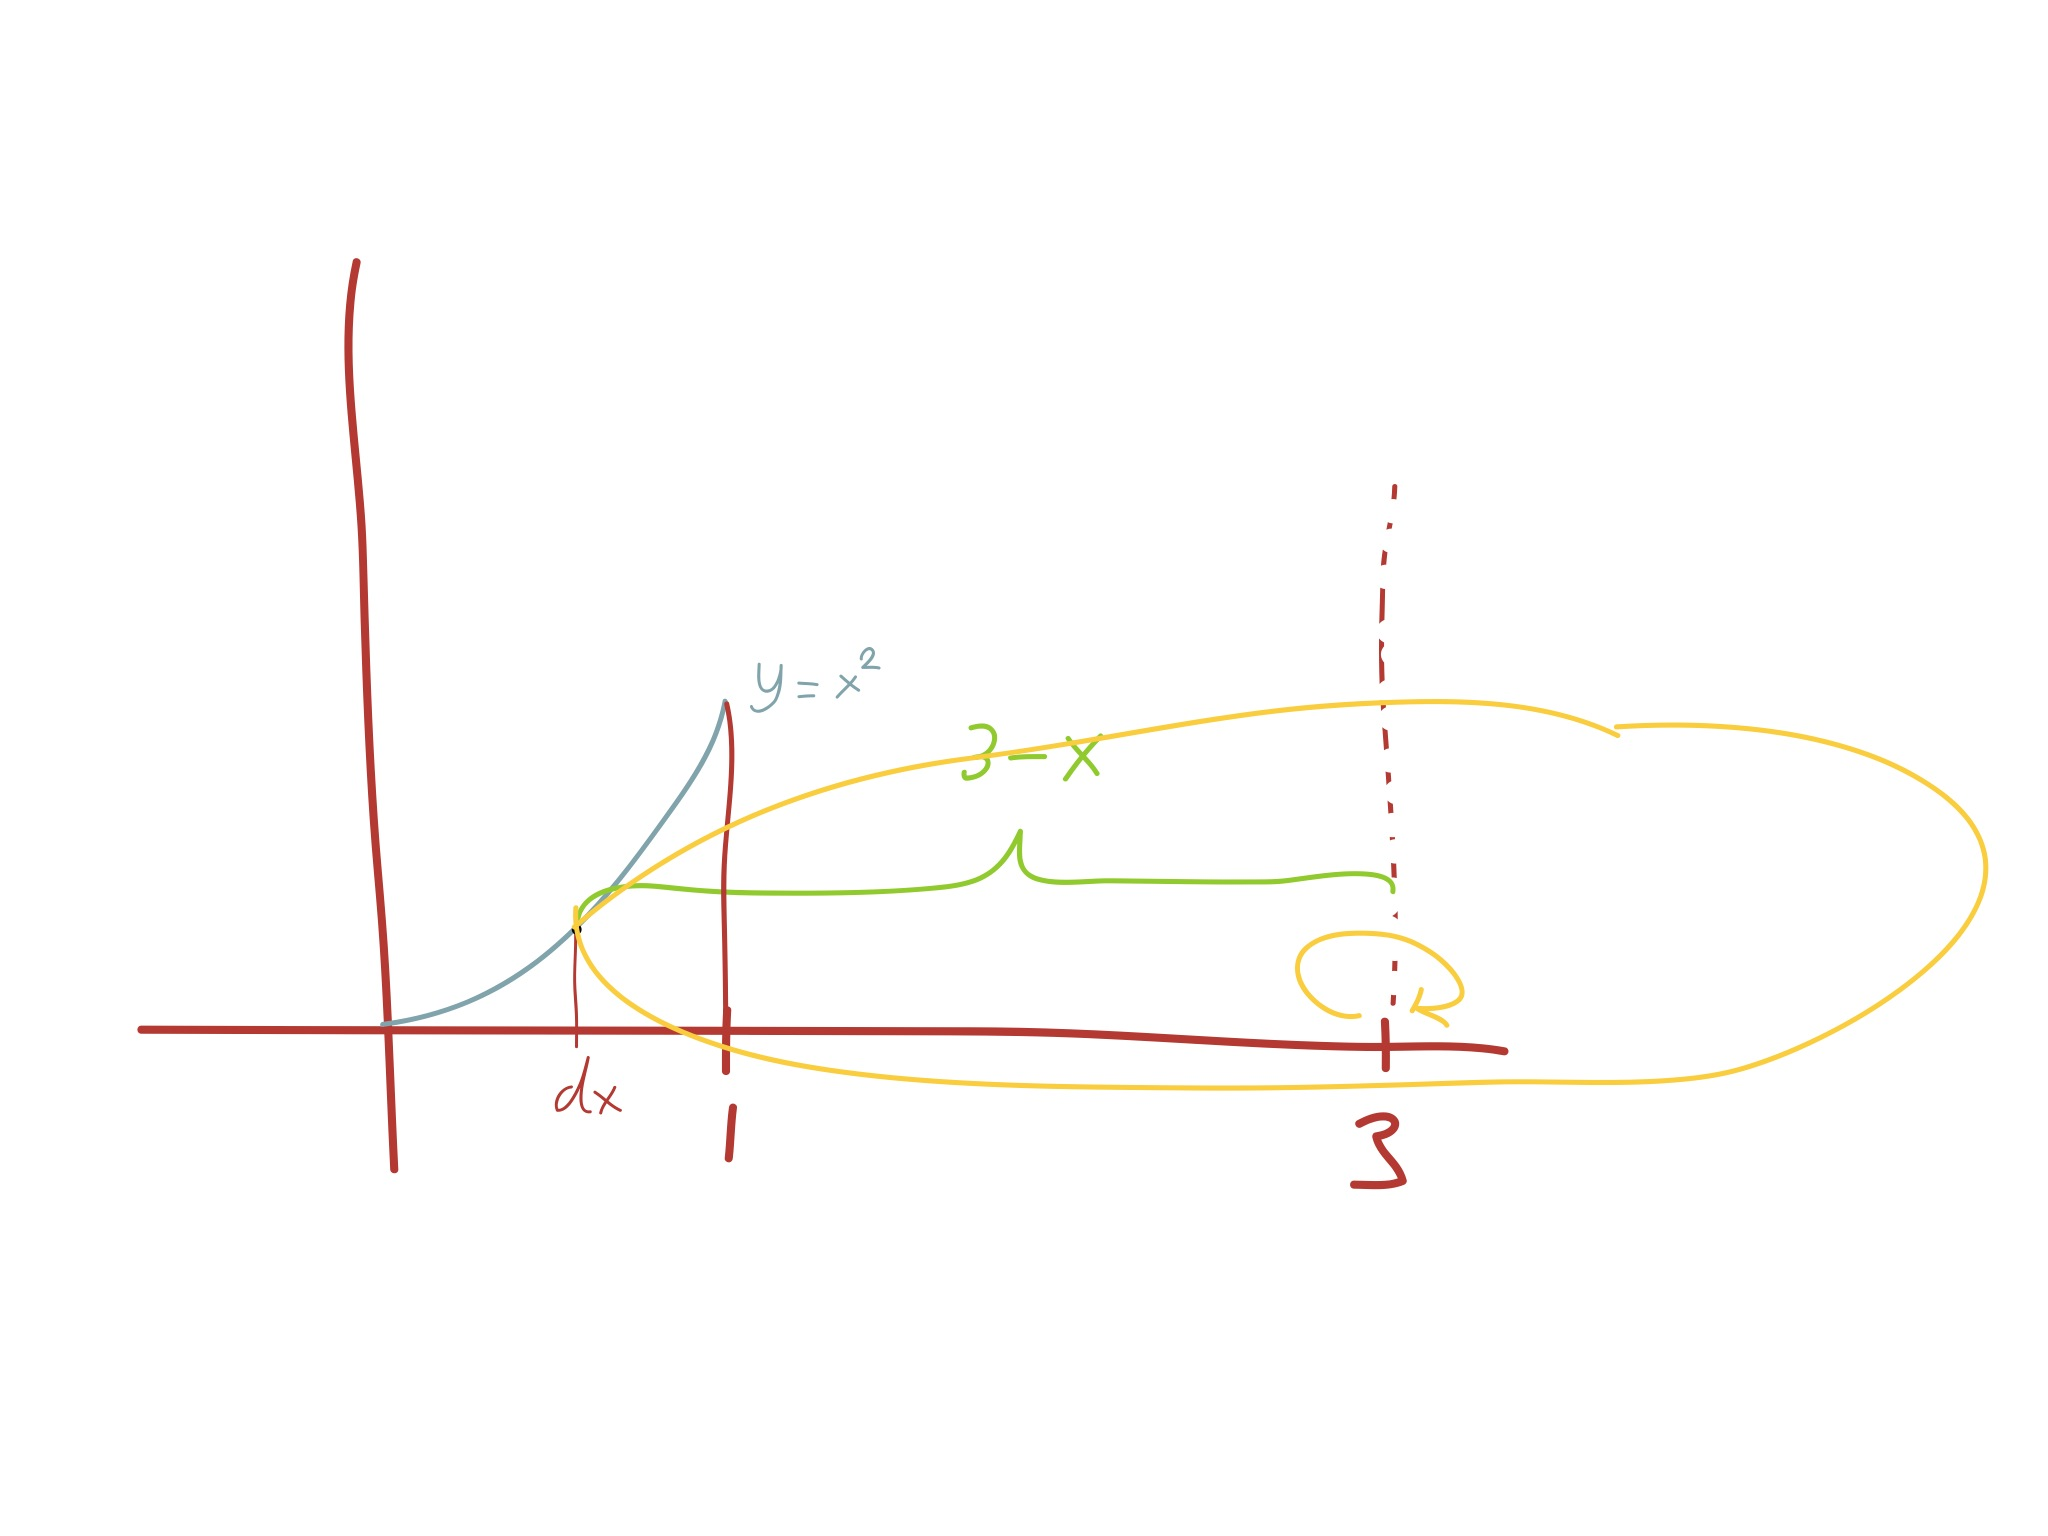
\includegraphics[scale=0.10]{img/img4.jpg}
$$T_x=(x, \f{f(x)}2) $$
$$dV = 2\pi x f(x) dx $$

Pappos-guldins regel för rotationsvolym:
$$ dV = tyngdpunktens\ vag * arean $$

\subsection{Ex 1}
Beräkna volymen av den kropp som uppkommer då

$$ D=\{ (x,y) : 0\le x\le 1, 0\le y\le x^2 \} $$
roteras kring linjen $x=3$

%img 5
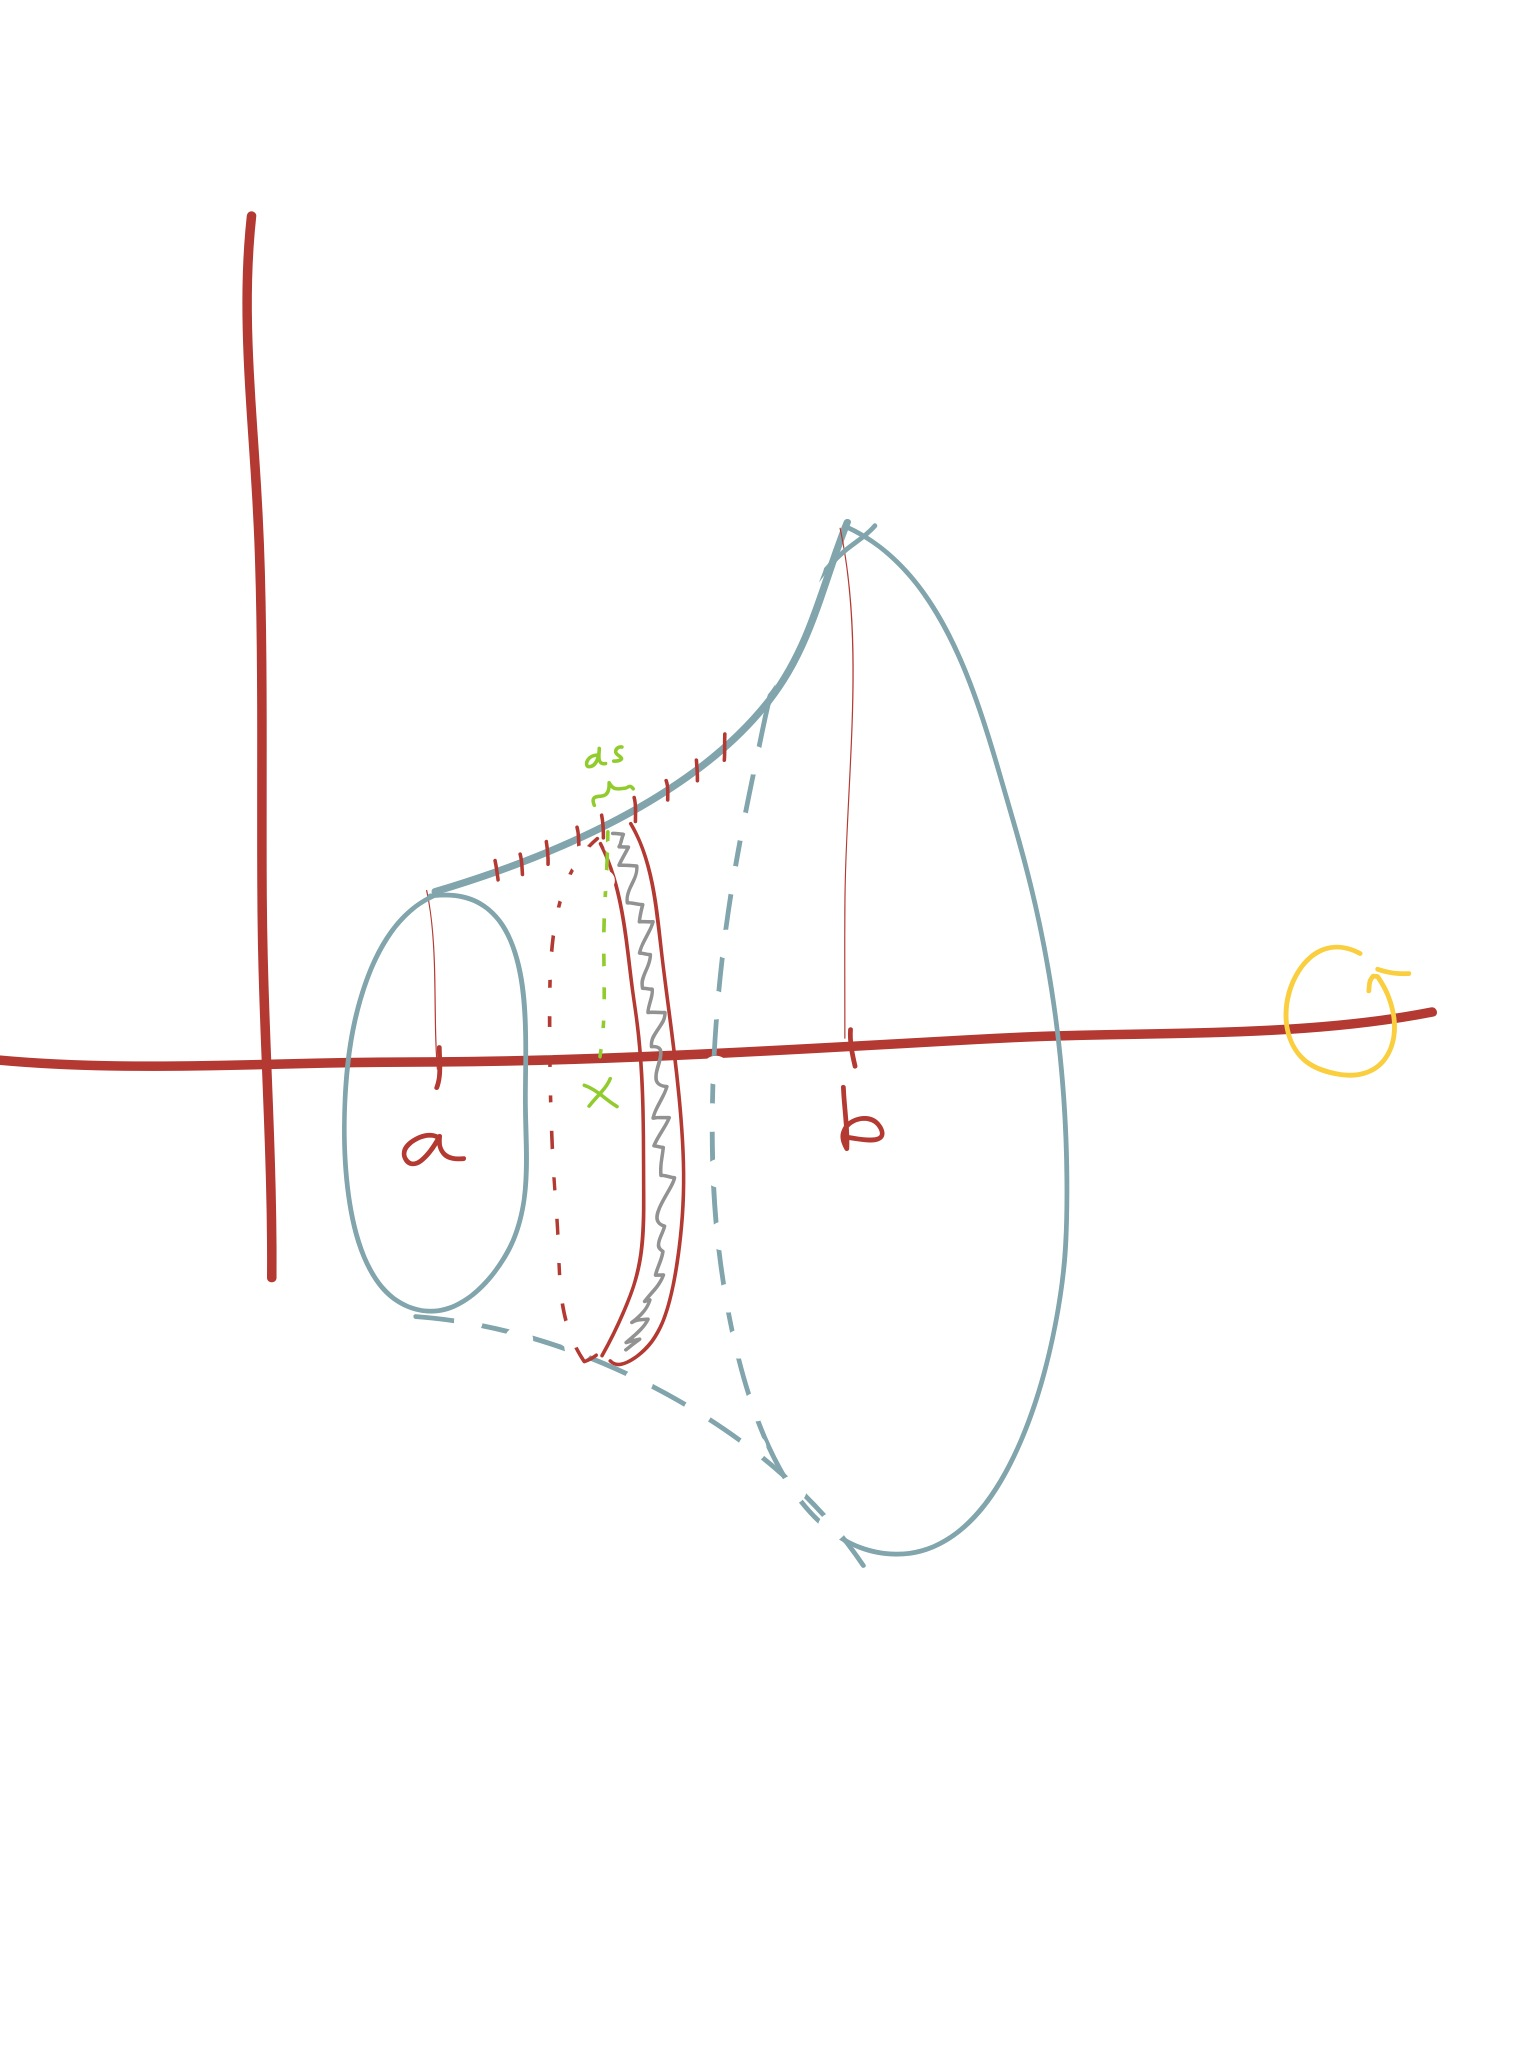
\includegraphics[scale=0.15]{img/img5.jpg}
$$T_x=(x, \f{x^2}2) $$
$$ dV= 2\pi(3-x)(f(x) dx)$$
$$ f(x) = x^2 $$
$$ dV= 2\pi(3-x)(x^2 dx)$$
$$ V=2\pi\int^1_0{(3-x)x^2dx}=2\pi\int_0^1{(3x^2-x^3)dx} = \dots = \f 32 \pi $$

\section{Rotationsarea}
$$ y=f(x), a\le x\le b, f, f' kontinuerliga $$
$$ dA = 2\pi f(x) ds \im A = \int_a^b dA = 2\pi \int^b_a f(x) ds =
\bra{ds = \sqrt{1+f'(x)^2} dx} =$$
$$A = 2\pi \int_a^b{f(x)\sqrt{1+f'(x)^2} dx} $$
Pappos-guldins regel för rotationsarea:
$$ dA=2\pi f(x) ds $$

\subsection{Ex 2}
Bestäm arean av den yta som uppkommer då
$ y=2x, 1\le 2\le 2 $ roteras ett varv kring linjen $y=-2$
% img 6
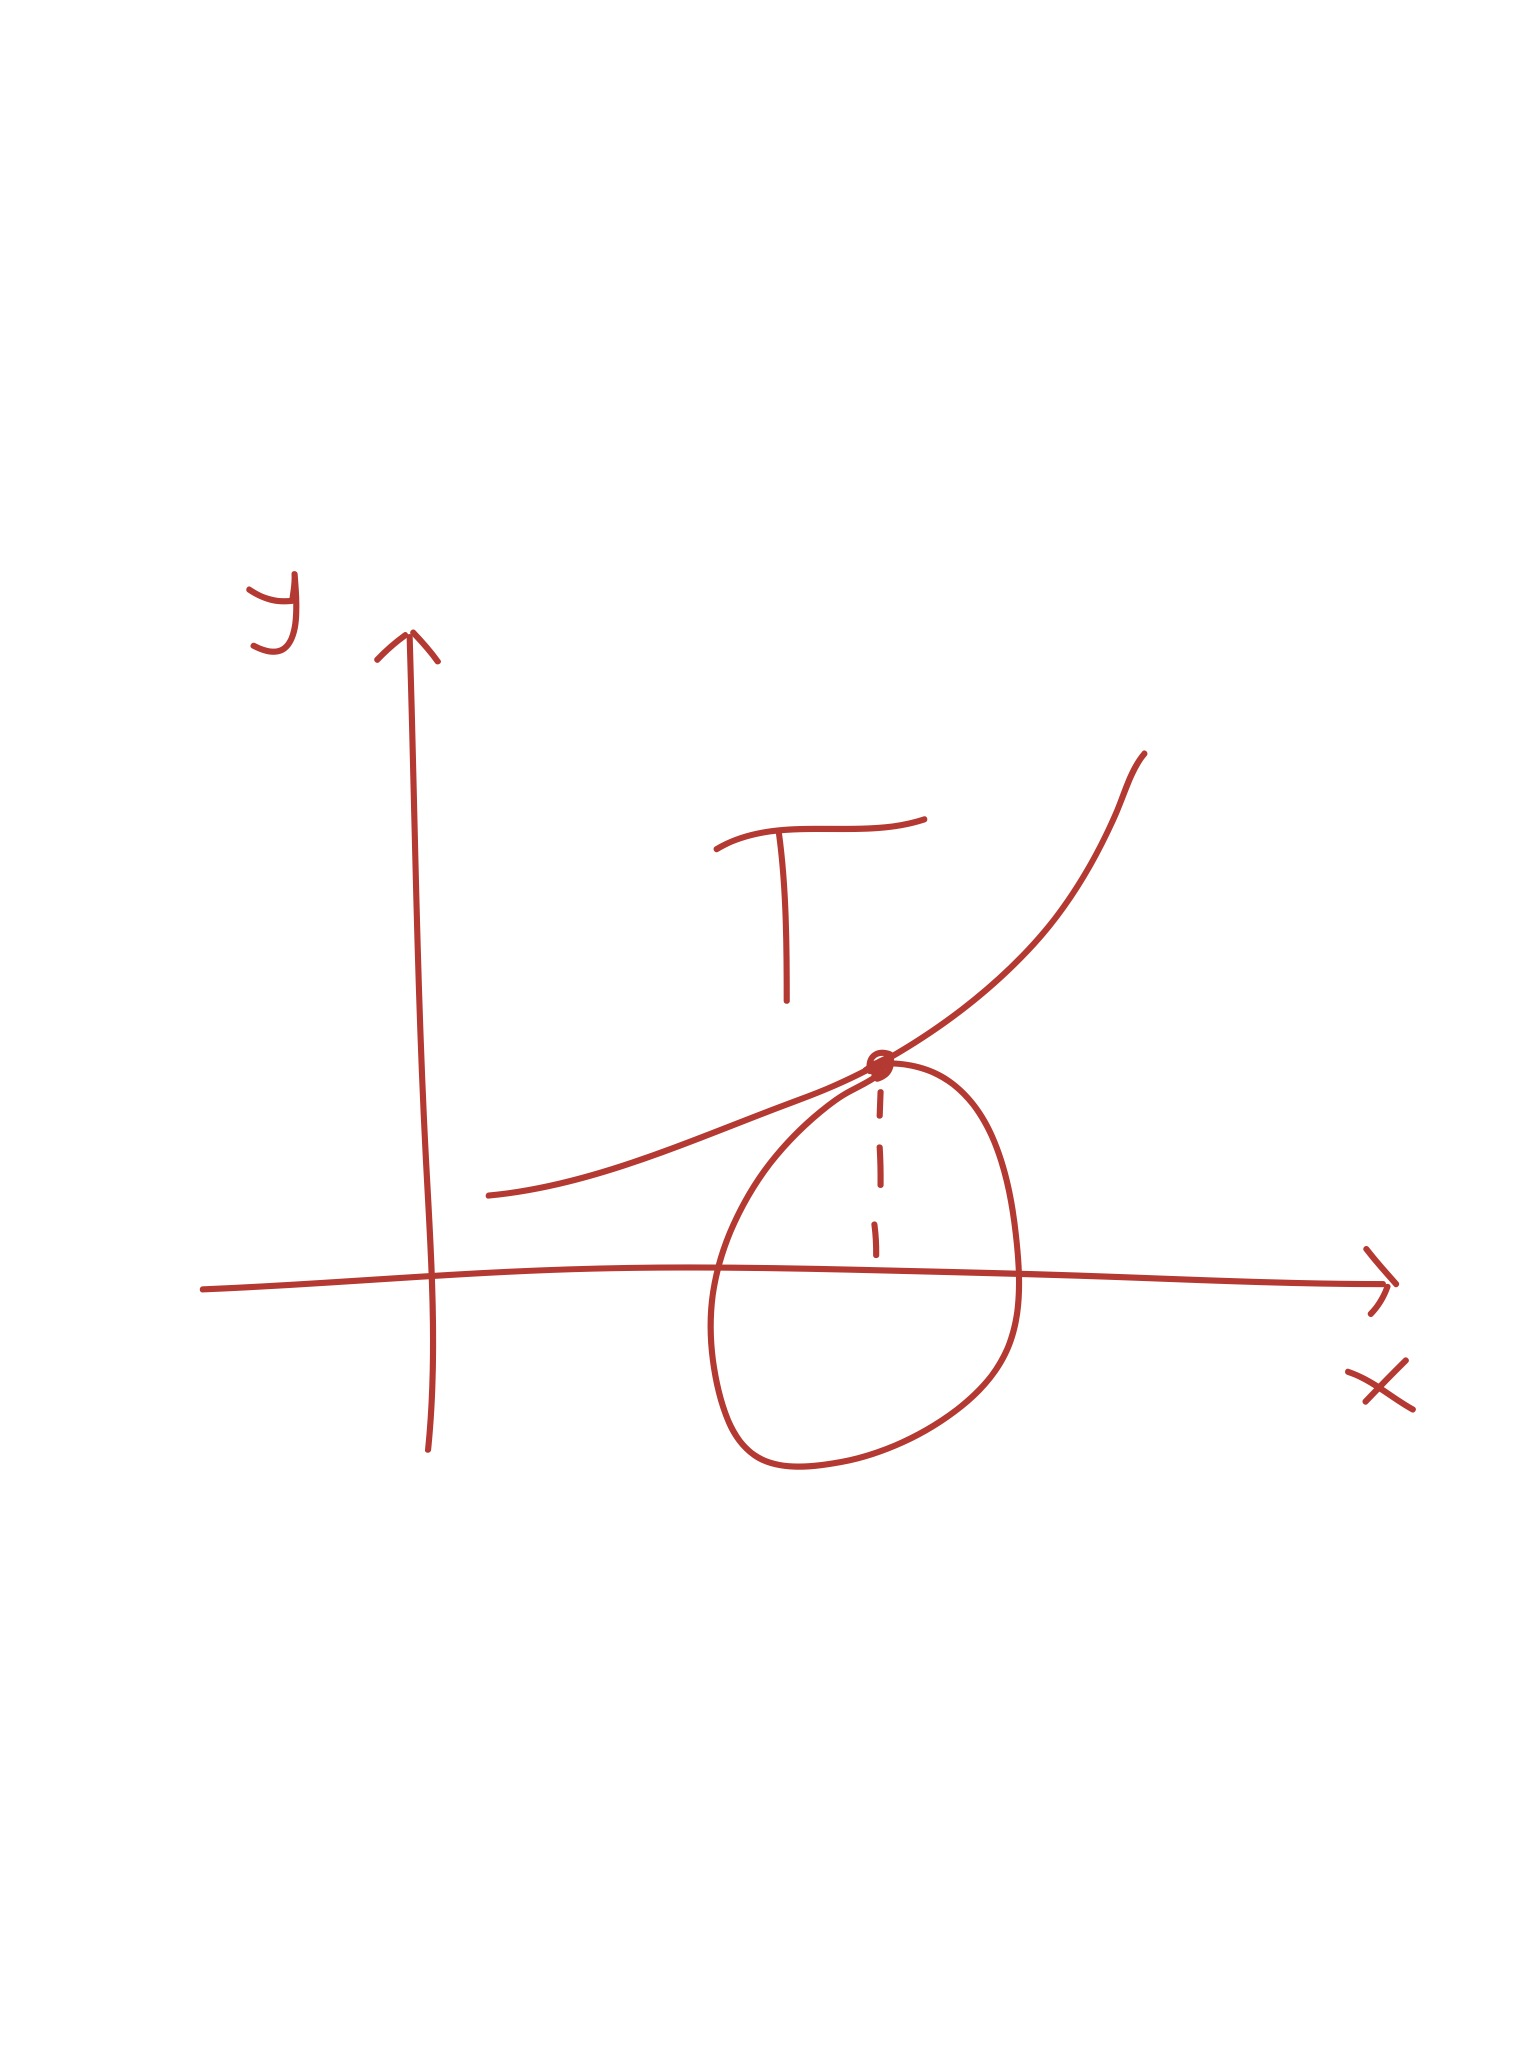
\includegraphics[scale=0.15]{img/img6.jpg}

$$ dA = 2\pi (f(x) + 2) ds = 2\pi (f(x) + 2) \sqrt{1+f'^2(x)} dx $$
$$ dA = 2\pi(2x+2)\sqrt{1+2^2} dx $$
$$ A=2\pi\int^2_1{(2x+2)\sqrt 5 dx} = 4\pi\sqrt 5\int^2_1{(x+1)dx} = 10\pi\sqrt 5 $$

\section{Tyngdpunkten}
$$ D-homogent p=1 $$
$$ m(D)=A(D) $$
$$ T=(x_T, y_T) $$
$$ M_y = x_Tm(D) = \int x dA \im x_T \int dA = \int xdA $$
$$ dM_y = xdA = xl(x)dx $$
$$ m(D) = \int dA $$
$$ x_T = \f{\int xdA}{\int dA} $$
% img 7
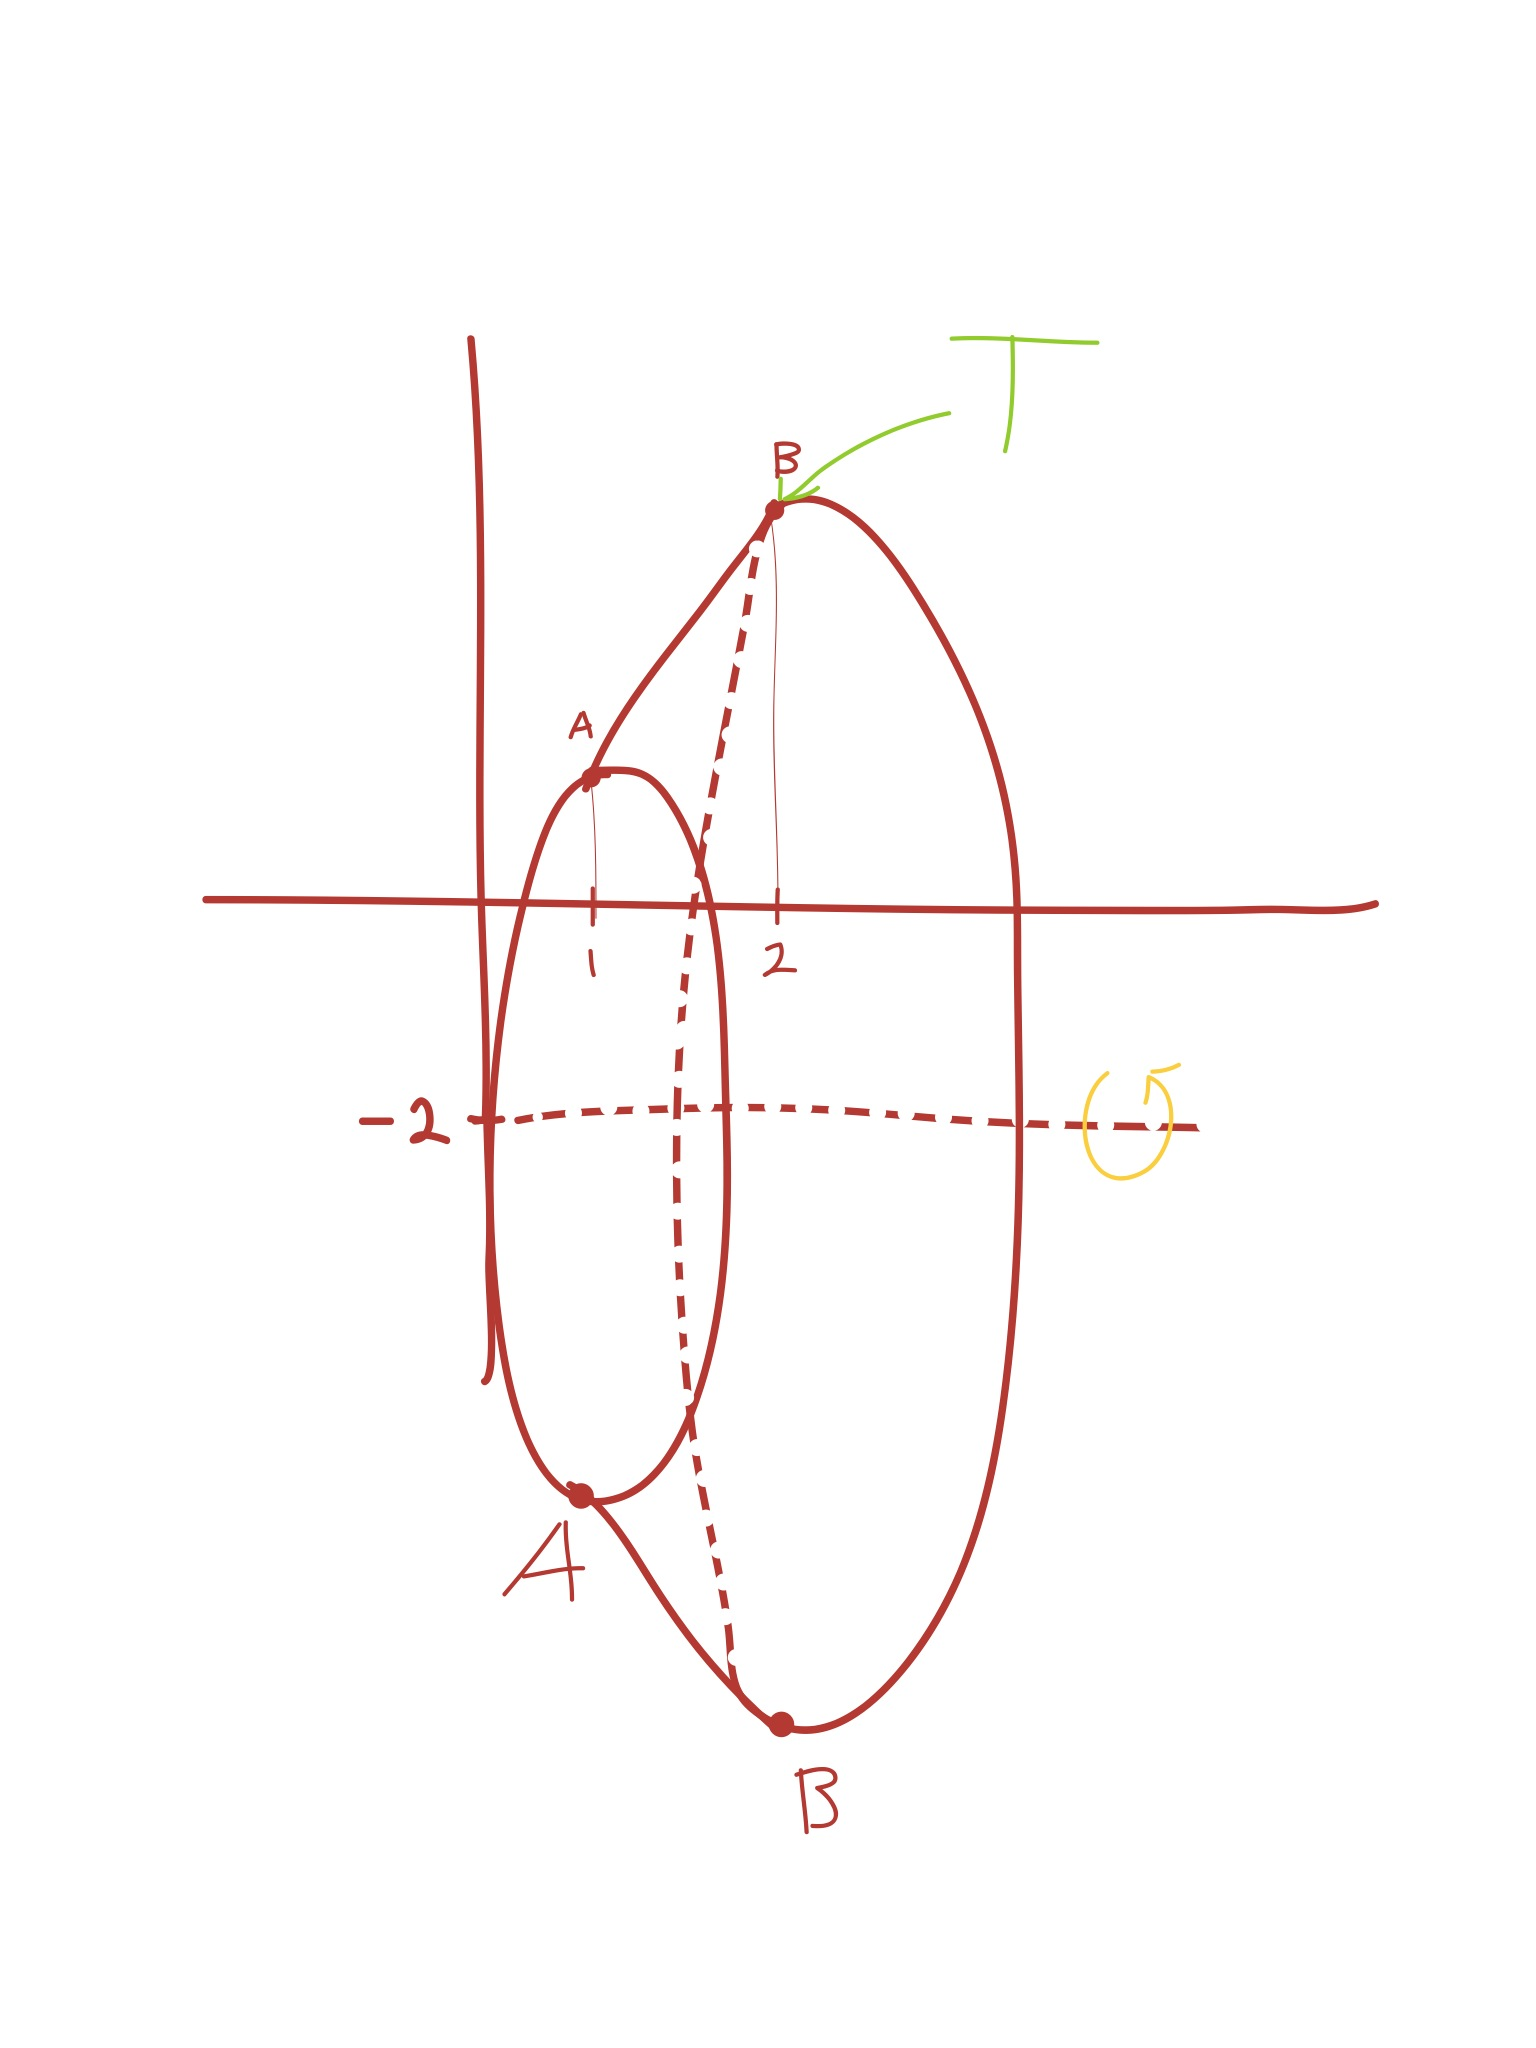
\includegraphics[scale=0.15]{img/img7.jpg}
$$ M_x = y_T \int dA = \int y dA $$
$$ dM_x = y dA $$
$$ y_T \int dA = \int y dA $$
$$ y_T = \f{\int y dA}{\int dA} $$
$$ dA = l(y) dy $$
$$ y_T = \f{\int yl(y) dy}{\int l(y) dy} $$
$$ T=\pa{\f{\int xdA}{\int dA}, \f{\int ydA}{\int dA}} $$

\subsection{}
% img 8
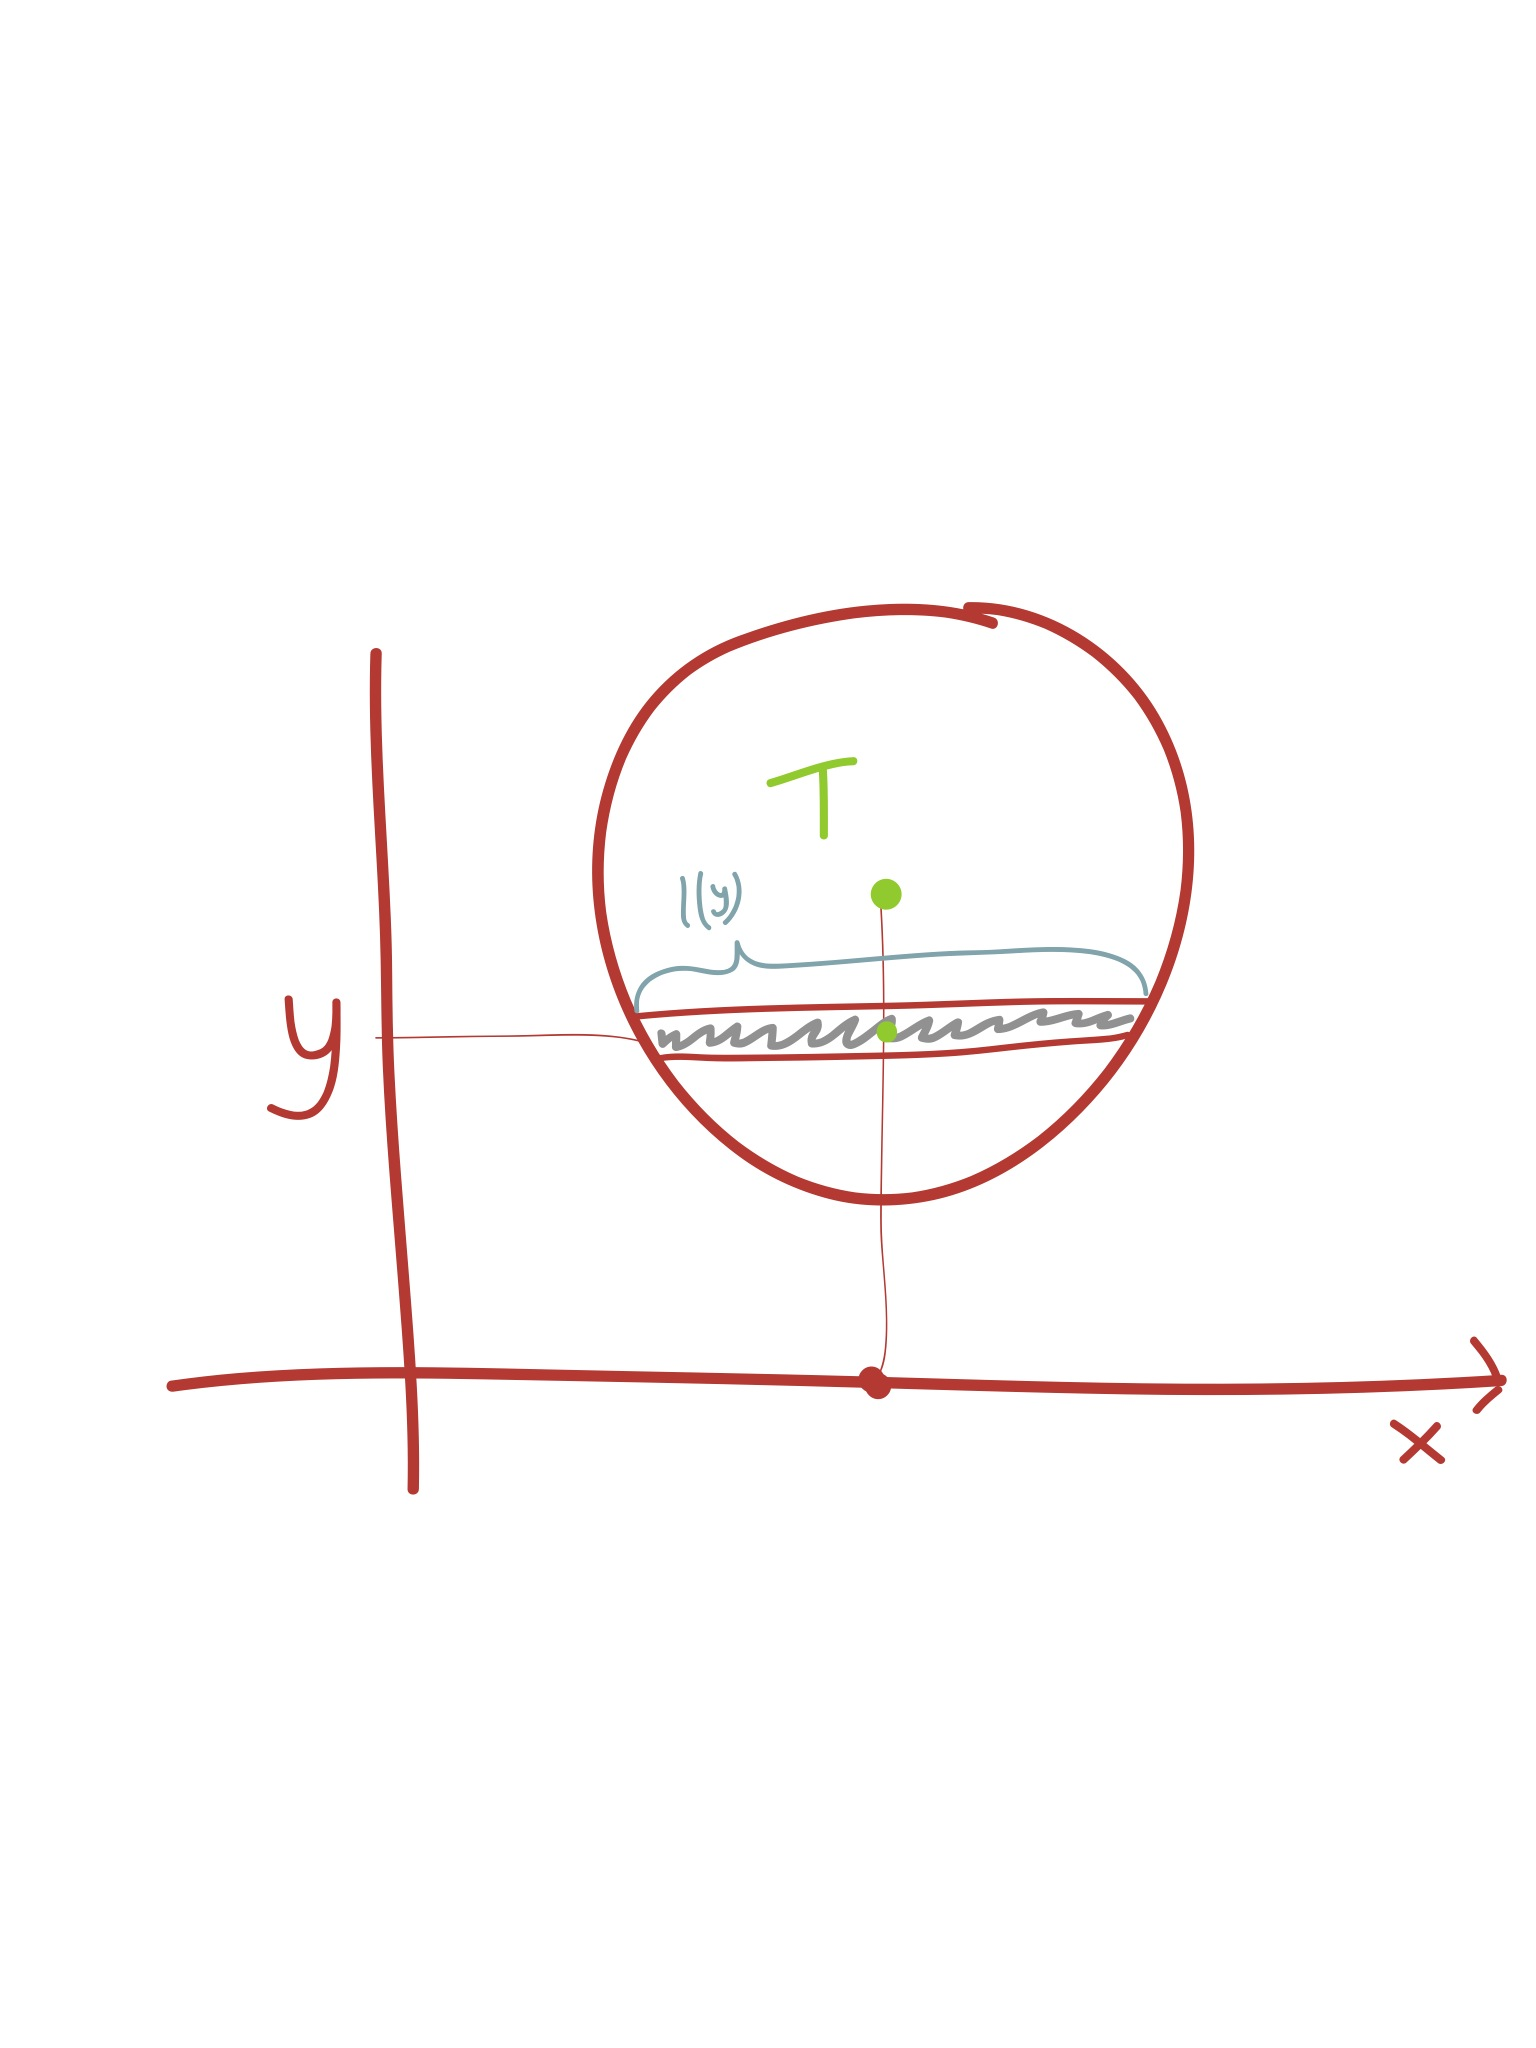
\includegraphics[scale=0.15]{img/img8.jpg}
$$ D=\{ (x,y) : a\le x\le b, g(x)\le y\le f(x) \} $$
$$ dA = (f(x) - g(x)) dx $$
$$ A=\int dA = \int^b_a (f(x) - g(x)) dx $$

$$ x_T\ \int^b_a(f(x)-g(x)) dx = \int^b_a xdA $$
$$ x_T\ \int^b_a(f(x)-g(x)) dx = \int x(f(x) - g(x)) dx $$

$$ x_T=\f{\int^b_a x(f(x) - g(x)) dx}{\int^b_a (f(x) - g(x)) dx}$$


$$ dM_x =\f{f(x)+g(x)}2dA = \f{f(x)g(x)}2(f(x) - g(x)) dx  $$
$$ y_T\ \int dA = \int dM_x $$
$$ \im y_T \int^b_a dA = \int^b_a{\f{f(x) + g(x)}2 (f(x) - g(x)) dx } $$
$$ y_T \int^b_a(f(x) - g(x)) dx = \f 12 \int^b_a(f^2(x) - g^2(x)) dx $$
$$ y_T = \f 12 \f{\int^b_a(f^2(x) - g^2(x)) dx}{\int^b_a{f(x) - g(x) dx}} $$

\subsection{Ex 3}
% img 9
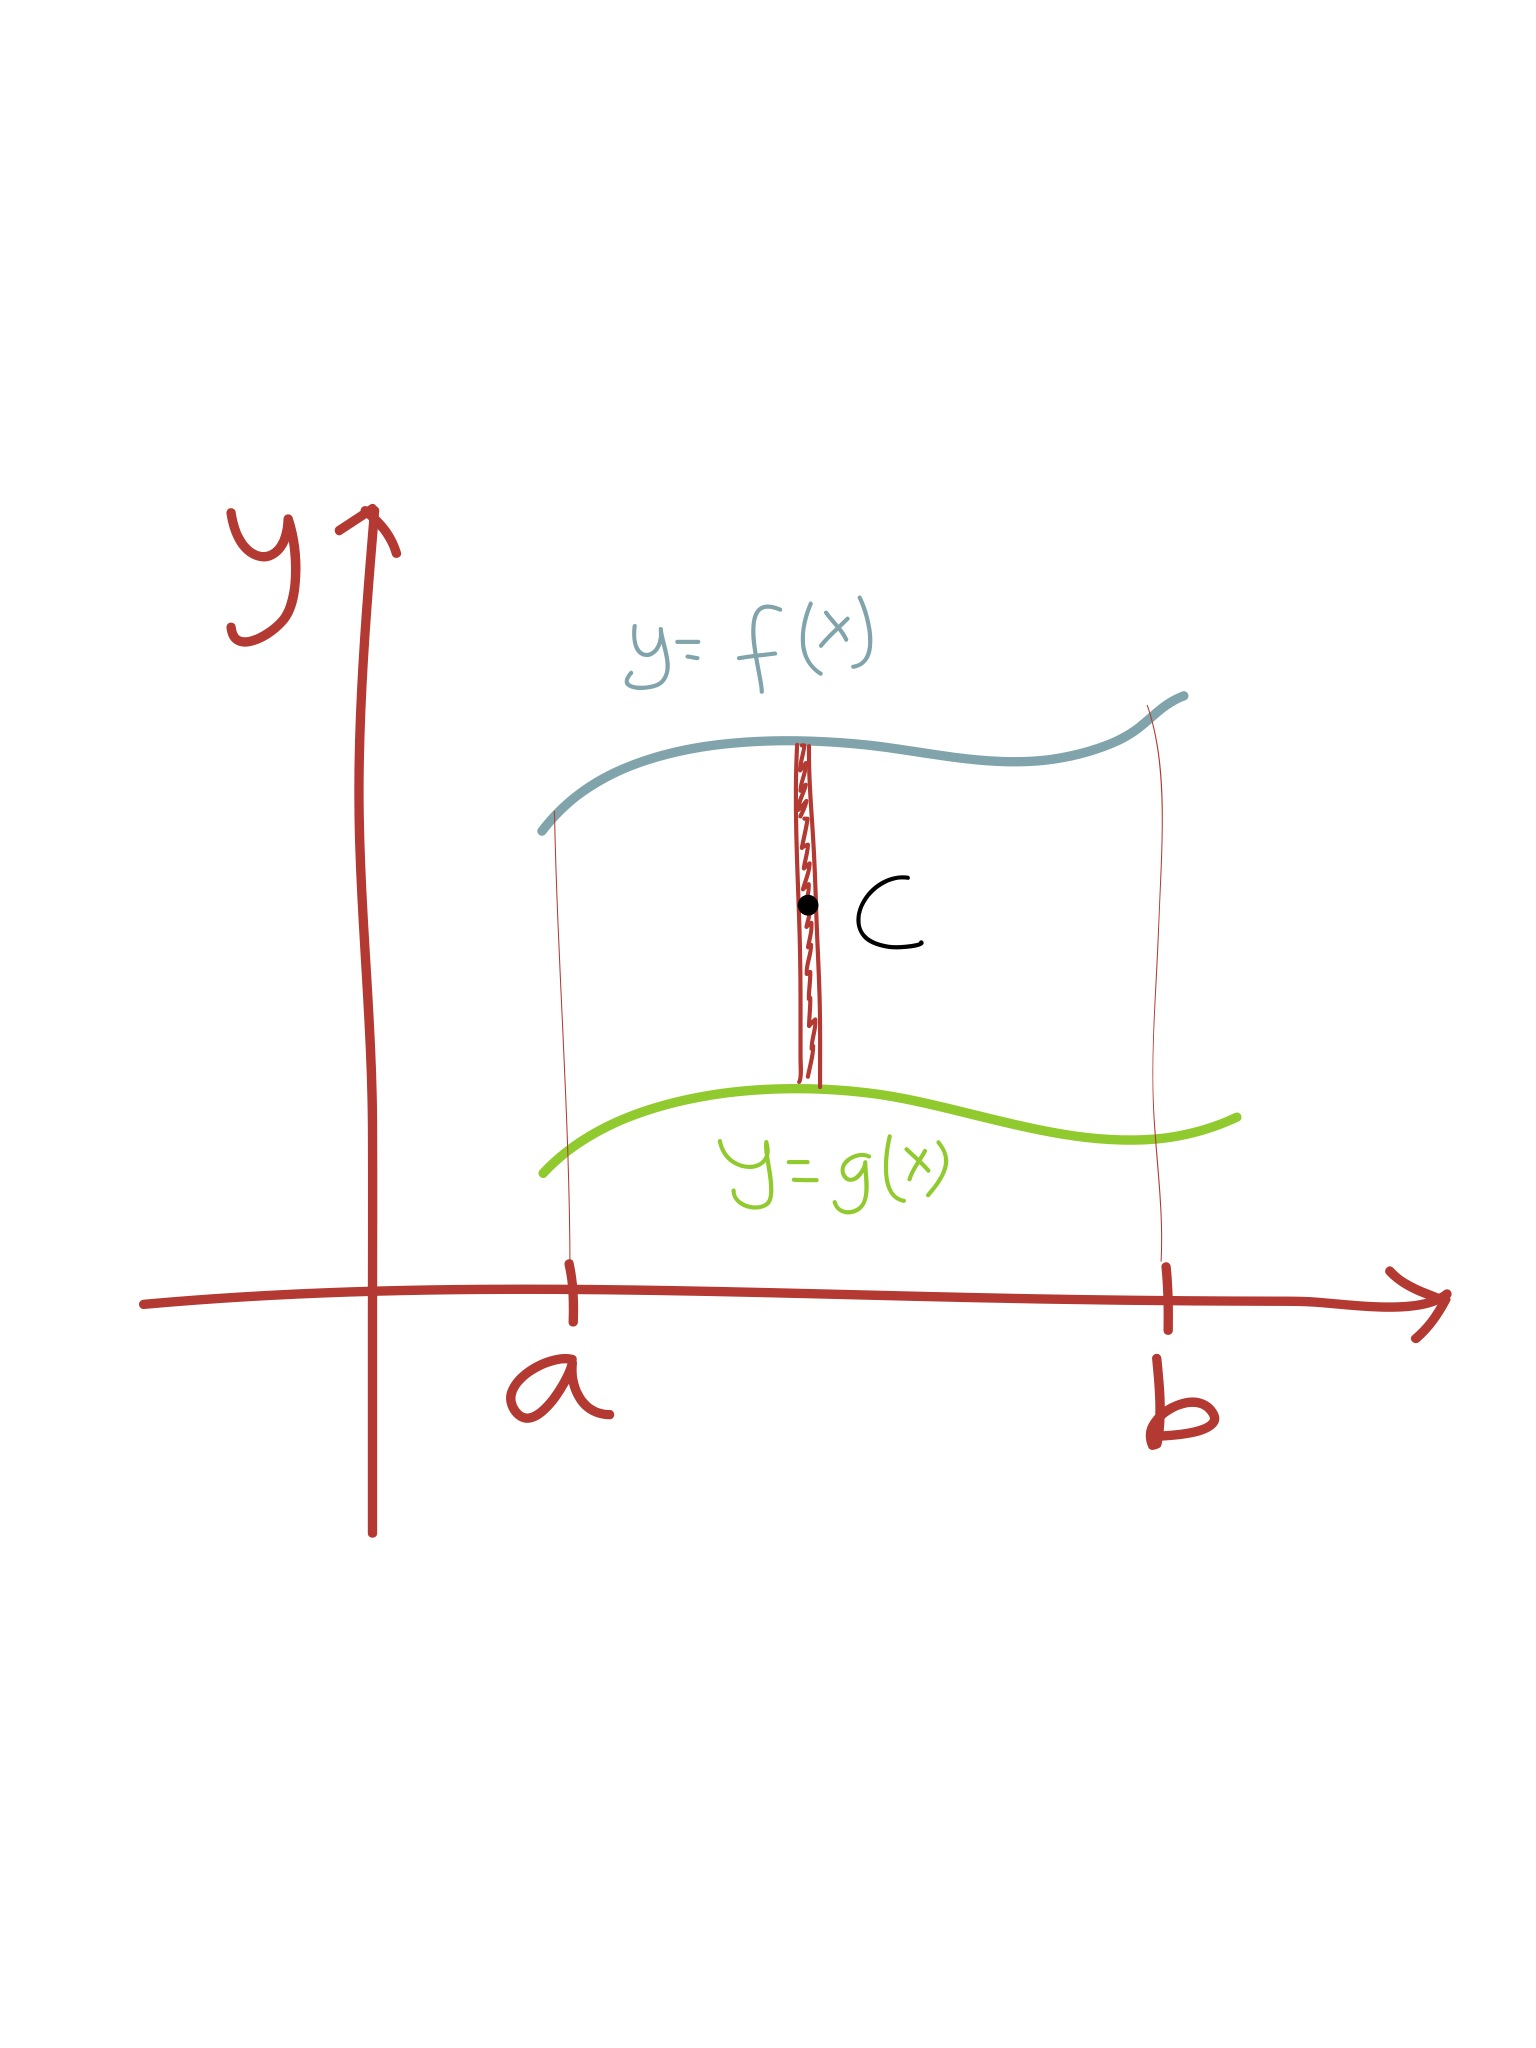
\includegraphics[scale=0.15]{img/img9.jpg}\\
$AB= 2a$ $\Delta OAB$ likbent homogen triangel
$$ T=(x_T, y_T); f(x)= \f ahx; g(x) = -\f ah x $$
$$ x_T = \f{\int^h_0{x2\f ah x dx}}{\int^h_0 2 \f ah x dx} = $$
$$ =\f{2\f ah \int^h_0{x^2 dx}}{2\f ah \int^h_0 xdx} =$$
% todo: buggy
$$ =\f{\bra{\f {x^3}3}^h_0}{\bra{\f{x^2}2}^h_0} = \f{\f 13 h^3}{\f 12 h^2} = \f 23 h; y_T = 0$$

\end{document}
